
\subsubsection{Feedforward Neural Networks}

Feedforward neural networks are a non-parametric estimator that can be used for classification and regression \cite{alpaydin}. They are called neural networks because they are formed by composing functions connected by a weight matrix. Each layers output is passed to the next layer thus forming a network. The activation functions can be thought of as "neurons" and the matrices as connections between them.

\begin{figure}[H]
\centering
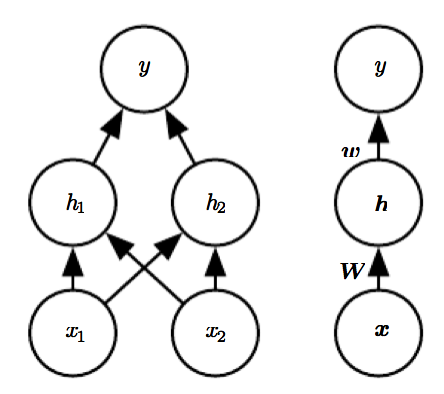
\includegraphics[width=0.4\textwidth]{images/nnet.png}
\caption{
  A depiction of a feedforward neural network drawn in two different styles. The circles are neurons and the lines between them connections between them. x and y are the input and output layers respectively. \cite{deep-learning-book}
}
\label{fig:nnet}
\end{figure}

Neural networks can be used to approximate functions such as probability distributions. However, as opposed to many linear models, neural networks can not be trained by using a closed form optimization method. The way they are trained is that a cost function is defined as the optimization goal. The cost is then minimized using gradient based learning. The backpropagation algorithm is used to update the weights and biases of the model to minimize the cost.

For neural networks, an online learning approach is typically used. Training examples are given in small batches which are evaluated against the cost function. The weights and biases are adjusted to minimize the cost function. Training in this fashion means that the training procedure does not have to store all of the training data in external memory. This makes neural networks well suited for problems with a lot of data.

In this paper we examine perhaps the most simple form of a feedforward neural network: a network with only fully connected layers. Fully connected layers are layers where the input is multiplied by a weight matrix, a bias term is added and the result is passed to some activation function. Typical activation functions include the sigmoid, tanh and restricted linear unit functions.

For classification we create a network with n neurons at the output layer where n is the amount of output classes. These neurons represent each of the output classes. At the output layer a softmax activation function is typically used. The softmax function outputs a n-dimensional vector that sums to one yielding what can be interpreted as a normalized probability distribution over the output classes. Categorical cross-entropy is used as the cost function to optimize the network.

For regression tasks linear activation functions are typically used and the output values are summed to yield the predicted value \cite{deeplearning4j-docs}. Mean squared error is often used to minimize the error of the network.

Neural networks are very versatile and can be used for a wide variety of problems. They also work very well in high dimensional settings. They are however computationally expensive to train. They also have quite a lot of parameters that can be tuned. This can make finding a good set of parameters time consuming. Grid search and other search techniques can however be used to help in the search \cite{deep-learning-book}.

\subsubsection{Random Forests}

Decision trees are a parametric method for supervised learning \cite{alpaydin}. The hypothesis is represented using a binary tree where at each node a binary decision is made. The training examples at the leaf nodes are used to make a prediction. For classification the most common training label at a leaf node represents the output class and for regression the labels for the training data are averaged to get the prediction.

Decision trees are learned by recursively expanding the tree using one of many learning algorithms available.

Random forests are an averaging based ensemble method specifically designed for decision trees \cite{sklearn}. Several models are trained by sampling with replacement from the training set. The predictions of each model is averaged to construct the final predictions. This way we can use several individual models with high variance and use averaging to reduce the overall variance. Decision trees typically can have high variance suffering from overfitting. They thus lend themselves very well for ensemble methods. Ensemble methods make use of this variance to reduce overfitting.

